\documentclass[14pt]{extbook}
\usepackage{multicol, enumerate, enumitem, hyperref, color, soul, setspace, parskip, fancyhdr} %General Packages
\usepackage{amssymb, amsthm, amsmath, bbm, latexsym, units, mathtools} %Math Packages
\everymath{\displaystyle} %All math in Display Style
% Packages with additional options
\usepackage[headsep=0.5cm,headheight=12pt, left=1 in,right= 1 in,top= 1 in,bottom= 1 in]{geometry}
\usepackage[usenames,dvipsnames]{xcolor}
\usepackage{dashrule}  % Package to use the command below to create lines between items
\newcommand{\litem}[1]{\item#1\hspace*{-1cm}\rule{\textwidth}{0.4pt}}
\pagestyle{fancy}
\lhead{Progress Quiz 1}
\chead{}
\rhead{Version A}
\lfoot{2654-6976}
\cfoot{}
\rfoot{Fall 2020}
\begin{document}

\begin{enumerate}
\litem{
First, find the equation of the line containing the two points below. Then, write the equation as $ y=mx+b $ and choose the intervals that contain $m$ and $b$.\[ (6, -10) \text{ and } (-11, -11) \]\begin{enumerate}[label=\Alph*.]
\item \( m \in [0.01, 0.09] \hspace*{3mm} b \in [9.3, 11.3] \)
\item \( m \in [0.01, 0.09] \hspace*{3mm} b \in [-10.7, -8.2] \)
\item \( m \in [0.01, 0.09] \hspace*{3mm} b \in [-0.4, 1.2] \)
\item \( m \in [-0.08, -0.04] \hspace*{3mm} b \in [-12.3, -11.3] \)
\item \( m \in [0.01, 0.09] \hspace*{3mm} b \in [-16.9, -13.4] \)

\end{enumerate} }
\litem{
Find the equation of the line described below. Write the linear equation as $ y=mx+b $ and choose the intervals that contain $m$ and $b$.\[ \text{Perpendicular to } 9 x + 4 y = 15 \text{ and passing through the point } (-7, -6). \]\begin{enumerate}[label=\Alph*.]
\item \( m \in [0.04, 0.75] \hspace*{3mm} b \in [2.2, 3.6] \)
\item \( m \in [1.16, 3.19] \hspace*{3mm} b \in [-5.8, -2] \)
\item \( m \in [0.04, 0.75] \hspace*{3mm} b \in [-5.8, -2] \)
\item \( m \in [0.04, 0.75] \hspace*{3mm} b \in [-0.1, 1.4] \)
\item \( m \in [-1.3, -0.24] \hspace*{3mm} b \in [-9.4, -7.9] \)

\end{enumerate} }
\litem{
Solve the equation below. Then, choose the interval that contains the solution.\[ -10(-17x + 14) = -15(3x + 4) \]\begin{enumerate}[label=\Alph*.]
\item \( x \in [-1.1, -0.78] \)
\item \( x \in [1.39, 1.75] \)
\item \( x \in [0.9, 0.98] \)
\item \( x \in [-0.69, 0.73] \)
\item \( \text{There are no real solutions.} \)

\end{enumerate} }
\litem{
Solve the linear equation below. Then, choose the interval that contains the solution.\[ \frac{-8x -5}{5} - \frac{-5x + 7}{4} = \frac{-9x -6}{8} \]\begin{enumerate}[label=\Alph*.]
\item \( x \in [-2, -1.7] \)
\item \( x \in [1.1, 4.2] \)
\item \( x \in [6.6, 8.1] \)
\item \( x \in [0, 1.5] \)
\item \( \text{There are no real solutions.} \)

\end{enumerate} }
\litem{
Write the equation of the line in the graph below in Standard form $Ax+By=C$. Then, choose the intervals that contain $A, B, \text{ and } C$.
\begin{center}
    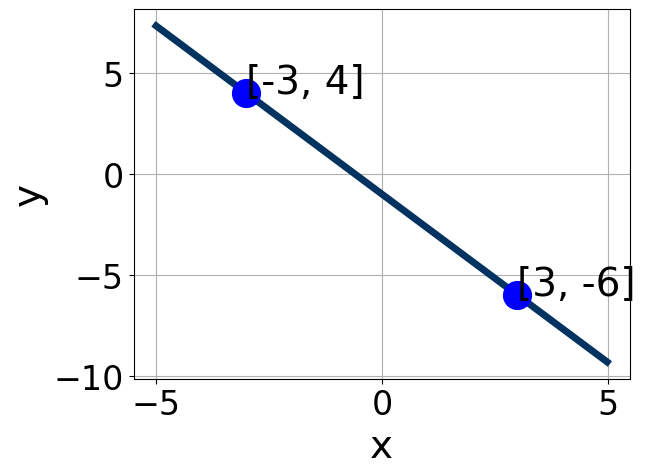
\includegraphics[width=0.5\textwidth]{../Figures/linearGraphToStandardCopyA.png}
\end{center}
\begin{enumerate}[label=\Alph*.]
\item \( A \in [-2.3, 0.7], \hspace{3mm} B \in [-0.5, 2.9], \text{ and } \hspace{3mm} C \in [0, 5] \)
\item \( A \in [-4.6, -2.3], \hspace{3mm} B \in [1.8, 5.8], \text{ and } \hspace{3mm} C \in [8, 14] \)
\item \( A \in [-2.3, 0.7], \hspace{3mm} B \in [-1.9, -0.3], \text{ and } \hspace{3mm} C \in [-7, 1] \)
\item \( A \in [0.3, 4.3], \hspace{3mm} B \in [1.8, 5.8], \text{ and } \hspace{3mm} C \in [8, 14] \)
\item \( A \in [0.3, 4.3], \hspace{3mm} B \in [-7.6, -1.1], \text{ and } \hspace{3mm} C \in [-11, -8] \)

\end{enumerate} }
\litem{
Solve the linear equation below. Then, choose the interval that contains the solution.\[ \frac{4x -3}{5} - \frac{-8x + 8}{7} = \frac{6x + 4}{3} \]\begin{enumerate}[label=\Alph*.]
\item \( x \in [-54.83, -50.83] \)
\item \( x \in [-1.49, 2.51] \)
\item \( x \in [-15.83, -12.83] \)
\item \( x \in [-262.5, -261.5] \)
\item \( \text{There are no real solutions.} \)

\end{enumerate} }
\litem{
Write the equation of the line in the graph below in Standard form $Ax+By=C$. Then, choose the intervals that contain $A, B, \text{ and } C$.
\begin{center}
    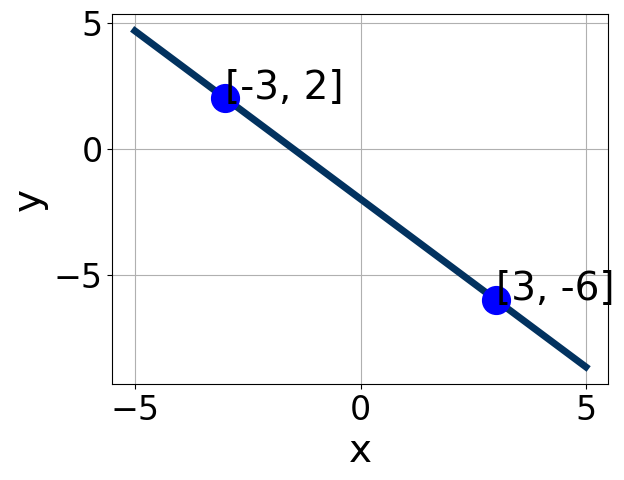
\includegraphics[width=0.5\textwidth]{../Figures/linearGraphToStandardA.png}
\end{center}
\begin{enumerate}[label=\Alph*.]
\item \( A \in [2.3, 6.9], \hspace{3mm} B \in [-6.2, -1.2], \text{ and } \hspace{3mm} C \in [4.97, 6.08] \)
\item \( A \in [-6.6, -3.6], \hspace{3mm} B \in [-6.2, -1.2], \text{ and } \hspace{3mm} C \in [4.97, 6.08] \)
\item \( A \in [0.3, 1], \hspace{3mm} B \in [-1.8, 0.6], \text{ and } \hspace{3mm} C \in [0.65, 1.54] \)
\item \( A \in [2.3, 6.9], \hspace{3mm} B \in [4.1, 6.2], \text{ and } \hspace{3mm} C \in [-6.72, -4.12] \)
\item \( A \in [0.3, 1], \hspace{3mm} B \in [0.8, 1.6], \text{ and } \hspace{3mm} C \in [-1.16, -0.54] \)

\end{enumerate} }
\litem{
First, find the equation of the line containing the two points below. Then, write the equation as $ y=mx+b $ and choose the intervals that contain $m$ and $b$.\[ (-5, -9) \text{ and } (-8, -6) \]\begin{enumerate}[label=\Alph*.]
\item \( m \in [-2.7, 0.9] \hspace*{3mm} b \in [12, 17] \)
\item \( m \in [-2.7, 0.9] \hspace*{3mm} b \in [-7, 0] \)
\item \( m \in [-2.7, 0.9] \hspace*{3mm} b \in [-17, -11] \)
\item \( m \in [-0.7, 1.9] \hspace*{3mm} b \in [1, 6] \)
\item \( m \in [-2.7, 0.9] \hspace*{3mm} b \in [1, 6] \)

\end{enumerate} }
\litem{
Solve the equation below. Then, choose the interval that contains the solution.\[ -2(-9x -5) = -12(-18x -8) \]\begin{enumerate}[label=\Alph*.]
\item \( x \in [0.52, 0.59] \)
\item \( x \in [-0.56, -0.48] \)
\item \( x \in [-0.46, -0.45] \)
\item \( x \in [-0.44, -0.37] \)
\item \( \text{There are no real solutions.} \)

\end{enumerate} }
\litem{
Find the equation of the line described below. Write the linear equation as $ y=mx+b $ and choose the intervals that contain $m$ and $b$.\[ \text{Perpendicular to } 8 x - 5 y = 6 \text{ and passing through the point } (-3, 7). \]\begin{enumerate}[label=\Alph*.]
\item \( m \in [-1.01, 0.54] \hspace*{3mm} b \in [-5.42, -4.85] \)
\item \( m \in [-0.36, 1.13] \hspace*{3mm} b \in [8.87, 9.3] \)
\item \( m \in [-1.01, 0.54] \hspace*{3mm} b \in [9.52, 10.75] \)
\item \( m \in [-1.01, 0.54] \hspace*{3mm} b \in [4.1, 5.25] \)
\item \( m \in [-1.89, -1.08] \hspace*{3mm} b \in [4.1, 5.25] \)

\end{enumerate} }
\end{enumerate}

\end{document}